\documentclass[a4paper, 10pt]{article}

\usepackage{graphicx}
\graphicspath{{images/}}
\usepackage{}
\usepackage{booktabs}
\usepackage{caption}
\usepackage[section]{placeins}
\usepackage{titlesec}

\usepackage{array}
\newcolumntype{C}[1]{>{\centering\arraybackslash}p{#1}}

\usepackage[table,xcdraw]{xcolor}
\usepackage{amsmath}
\usepackage{amsfonts}
\usepackage{amssymb}
\usepackage{hyperref}
\usepackage{graphicx}
\usepackage{subcaption}
\usepackage[a4paper, top=2cm, bottom=2cm, left=2cm, right=2cm]{geometry}
\setcounter{secnumdepth}{4}
\titleformat{\paragraph}
{\normalfont\normalsize\bfseries}{\theparagraph}{1em}{}
\titlespacing*{\paragraph}
{0pt}{3.25ex plus 1ex minus .2ex}{1.5ex plus .2ex}

\begin{document}
\begin{titlepage}
    \begin{figure}[ht]
        \centering
        
\includegraphics[width=\textwidth]{0-ise-logo.png}
    \end{figure}
    {\large \textit{Industrial Robot Project Report 2147308} \par}
    
    \vspace{1cm}
    {\huge \textbf{Project: Pick up box} \par}
    \vspace{1cm}
    
    {\large \textit{By} \par}
    \vspace{1cm}
    {\large \textbf{Thanakorn Sappakit, Nunnapat Anupongongarch, Tibet Buramarn, Thitaya} \par} 
    {\large \textbf{Divari, Tinapat Limisila, Chanapa Anuwatvimol, Tunyaluck Liengkorsakul} \par}
    \vspace{1cm}
    {\large Robotics \& AI Program, International School of Engineering, Chulalongkorn University \par}
    {\large 254 Phayathai Rd, Wang Mai, Pathum Wan, Bangkok, Thailand 10330 \par}
    
    \thispagestyle{empty}
    
    \begin{center}
        \item\section*{Abstract}
    \end{center}
    \large This report documents the development of an autonomous pick-and-place robotic system created as a term project for the Industrial Robots course. The system integrates a Universal Robots UR3 robotic arm with National Instruments’ Vision Builder software to detect, track, and retrieve boxes from a moving conveyor belt. Real-time communication between components is facilitated using TCP/IP sockets, while a Python-based control framework synchronizes the vision system, robotic arm, gripper, and conveyor belt. Key features include predictive positioning to account for system delays, adaptive gripper control based on object dimensions, and precise coordination across hardware and software. The system achieved the fastest picking performance among all groups at 2.7 seconds, demonstrating the practical effectiveness of robotics and vision integration in industrial automation.
    
    \begin{center}
        \item\section*{Keyword}
    \end{center}
    \textit{Industrial automation, UR3 robotic arm, computer vision, pick-and-place robot, TCP/IP communication, NI Vision Builder, predictive control, real-time systems, robotic integration, conveyor belt tracking.}


    
\end{titlepage}
\newpage
\tableofcontents

\newpage
\section{Introduction}
The integration of robotics and computer vision is increasingly vital in industrial automation, enhancing productivity. This report presents a detailed overview and analysis of our term project on Industrial Robots, “Pick Up Box,” an autonomous robotic system designed to pick objects from a moving conveyor belt. Employing the Universal Robots’ UR3 robotic arm coupled with the National Instruments’ Vision Builder software, the system reliably detects, tracks, and manipulates boxes positioned on the conveyor. The primary objective is to demonstrate the quick and efficient pick of a box through real-time coordination between the robotic arm and the vision system. This report elaborates on the system specifications, methodologies, TCP/IP communication, software architecture, and performance considerations.
\section{Specifications}
In this project, a robotic arm is tasked with detecting and picking up one of two boxes as they move slowly along a conveyor belt. The system uses a camera to detect the presence of a box, after which the robot automatically grabs it. The robotic arm starts at the midpoint of the conveyor belt, with its base coordinates defined in Table \ref{tab:specs}.

\renewcommand{\arraystretch}{1.1}
\begin{table}[h]
    \centering
    \caption{Project Specifications}
    \begin{tabular}{|C{7cm}|C{7cm}|}
        \hline
        \textbf{Specifications} & \textbf{Value} \\
        \hline
        Xbase   & 116 mm   \\
        \hline
        Ybase     & -300 mm     \\
        \hline
        Zbase & 80 mm \\
        \hline
        Rxbase   & 2.233 rad   \\
        \hline
        Rybase   & 2.257 rad \\
        \hline
        Rzbase      & -0.039 rad   \\
        \hline
    \end{tabular}
    \label{tab:specs}
\end{table}

After the first box passes the midpoint, a second box is placed at the far right end of the conveyor. This box will also be detected, grasped, and lifted by the robot to at least the height of its initial position. The second box is positioned randomly on the belt but aligned along the conveyor belt axis, with an orientation deviation of no more than $\pm 10^\circ$.

\section{Methodology}
This project integrates a UR3 robotic arm with a vision system and conveyor belt for autonomous pick-and-place operations. The system uses TCP/IP communication to transmit coordinates and commands between the robot, gripper, and conveyor. A Python-based control loop manages the synchronization between the vision system, robot, and conveyor, ensuring precise box detection and positioning. The vision system detects the position of boxes, and the robot arm moves accordingly to pick and place the objects.

The software implementation involves a custom Robot class for controlling the UR3 arm, which simplifies movement commands by using absolute pose instructions. The system accounts for delays, such as camera-to-computer latency, by predicting future box positions. Extensive testing was conducted to ensure accurate box detection, robot arm movements, and gripper functionality. This methodology enables reliable and efficient robotic operations within a dynamic environment.

\newpage
\section{TCP Communication}
A widely adopted communication method for interfacing with Universal Robots is the use of TCP/IP socket connections over Ethernet. This approach is favored for its simplicity and reliability. Universal Robots support several built-in Remote Control Servers including the Primary, Secondary, Real-time, and Dashboard servers all of which operate using the TCP/IP protocol. These servers are designed to receive and process remote commands from client applications running on external devices or other robotic systems, enabling seamless remote operation and integration.

The integration of TCP/IP socket communication in the UR3 robotic system provides a remote control and data exchange across all components including robot arm, gripper, vision system, and conveyor. Leveraging Python’s socket programming capabilities, the system establishes reliable channels for real-time command execution and sensor feedback, ensuring high accuracy and repeatability in industrial pick-and-place applications.

\begin{figure} [!ht]
    \centering
    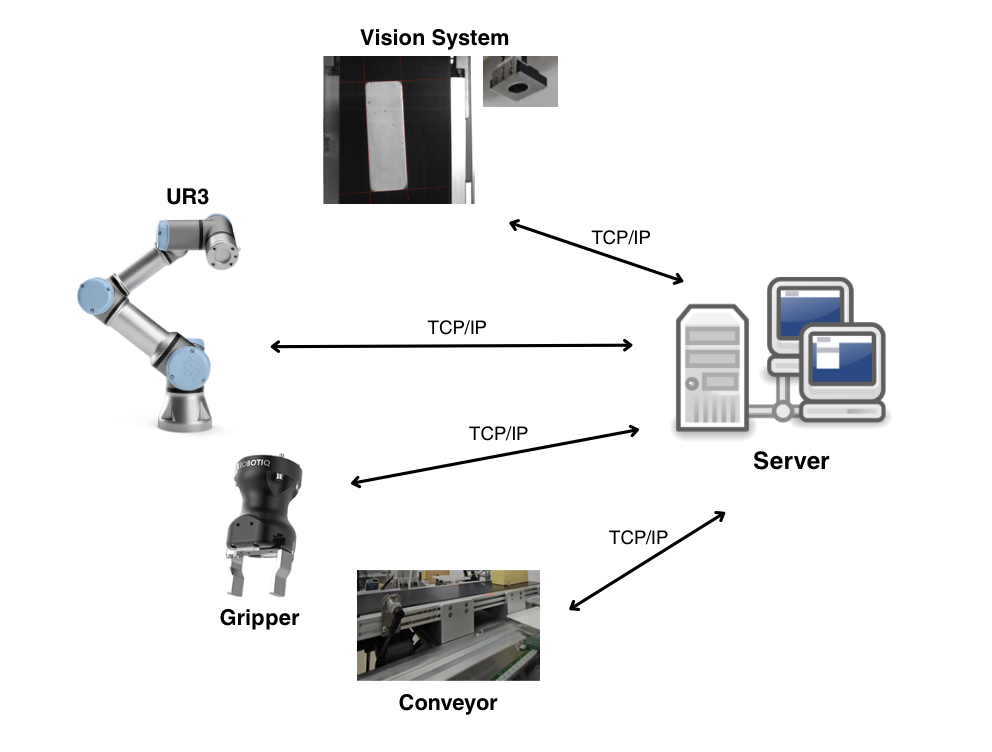
\includegraphics[width=\textwidth]{1-tcp.png}
    \captionsetup{justification=centering}
    \caption{TCP Communication between Components}
    \label{fig:1-tcp}
\end{figure}

By adopting this architecture, developers can interface with the UR3 and external vision systems and dynamic task coordination. The use of TCP/IP not only enhances communication reliability but also simplifies integration with other industrial devices, making it ideal for modular, remote-controlled robotic systems.

\newpage
\section{Vision Builder}
NI Vision Builder is a software tool developed by National Instruments (NI) \cite{ni_vbai}. It is used to create and run machine vision applications without writing code. It provides a step-by-step, menu-based interface to help users build vision inspection systems quickly. For our project, we use NI Vision Builder 2019 to manage our box detection pipeline before signaling the UR3 arm to pick up the box. Figure \ref{fig:3-vi} shows the complete pipeline for box detection in NI Vision Builder. Our pipeline consists of five main stages: Image Acquisition, Apply Filter, Define ROI, Edge Detection, and TCP Communication.

\begin{figure} [!ht]
    \centering
    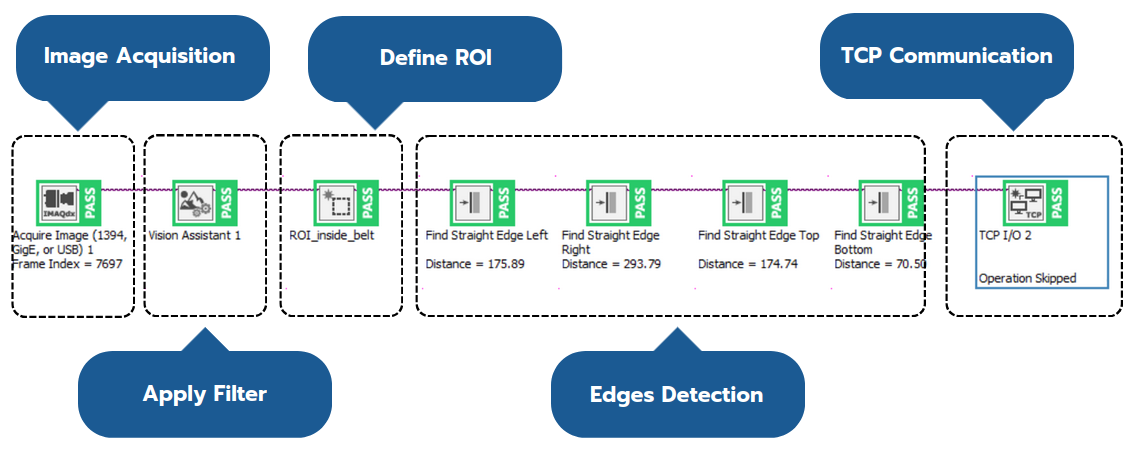
\includegraphics[width=\textwidth]{3-vi.png}
    \captionsetup{justification=centering}
    \caption{NI Vision Builder pipeline for box detection}
    \label{fig:3-vi}
\end{figure}

The first step of our pipeline is to acquire the image. We then apply a filter by slicing the image in the luminance plane from the HSL color format. This results in a black and white image, which is more suitable for image processing and edge detection. Figure \ref{fig:4-both} shows the image captured by the camera on the left and the same image after filtering on the right.

\begin{figure}[h!]
    \centering
    \begin{subfigure}[b]{0.45\textwidth}
        \centering
        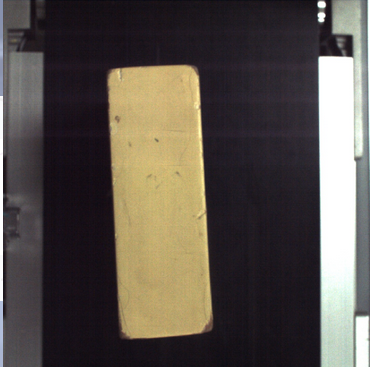
\includegraphics[width=\textwidth]{4-left.png} % Replace with your image file
        \caption{Image acquired by the camera}
    \end{subfigure}
    \hfill
    \begin{subfigure}[b]{0.45\textwidth}
        \centering
        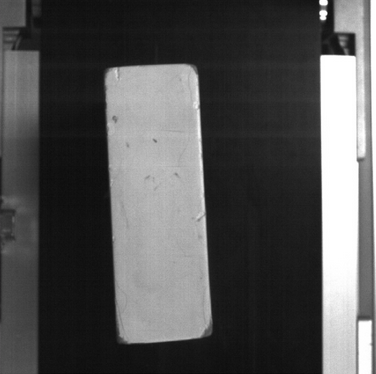
\includegraphics[width=\textwidth]{4-right.png} % Replace with your image file
        \caption{Image after applying the filter}
    \end{subfigure}
    \captionsetup{justification=centering}
    \caption{Comparison of the original image (left) and the filtered image (right)}
    \label{fig:4-both}
\end{figure}

For the third step, we define our ROI (Region of Interest) to be within the belt area. This serves two purposes: first, to prevent false edge detection outside the belt; and second, to reduce the size of the working image, thereby decreasing processing time. Figure \ref{fig:5-roi} shows our ROI, labeled in green on the image.

\begin{figure} [!ht]
    \centering
    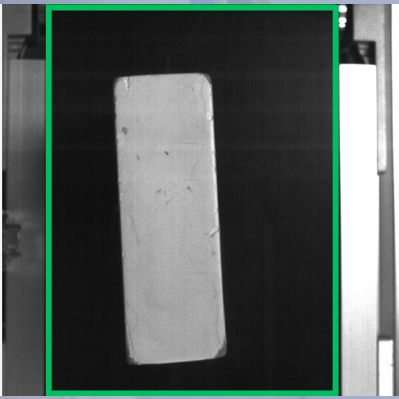
\includegraphics[width=0.5\textwidth]{5-roi.png}
    \captionsetup{justification=centering}
    \caption{ROI used in our pipeline, labeled in green}
    \label{fig:5-roi}
\end{figure}

\newpage
The next step in our pipeline involves detecting the box. We achieve this by identifying each edge, top, bottom, left, and right, separately using the ‘’Find Straight Edge tool’’ in NI Vision Builder. For each edge, we configure the search direction from the outer region towards the inner part of the box and set the edge polarity to detect transitions from dark to bright. This configuration allows us to accurately locate the outer edges of the box. The tool provides output metrics, specifically the x and y coordinates of two points defining each detected edge. Figure \ref{fig:6-edges} shows an example of edges detected using Find Straight Edge tool. Finally, we transmit these results via TCP communication in the following format:

\begin{center}
    \begin{verbatim}
        left_x1, left_y1, left_x2, left_y2 /
        right_x1, right_y1, right_x2, right_y2 /
        top_x1, top_y1, top_x2, top_y2 /
        bottom_x1, bottom_y1, bottom_x2, bottom_y2 |
    \end{verbatim}
\end{center}

\begin{figure} [!ht]
    \centering
    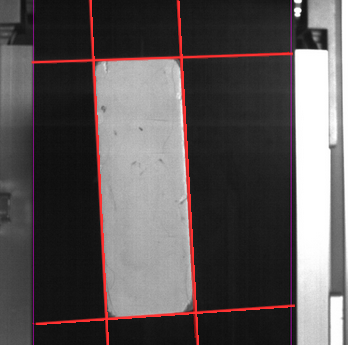
\includegraphics[width=0.5\textwidth]{6-edges.png}
    \captionsetup{justification=centering}
    \caption{Four edges of the box detected, labeled in red}
    \label{fig:6-edges}
\end{figure}

\newpage
\section{UR3 Arm}
In this project, we utilize the UR3 robotic arm. The UR3 is a compact, 6-degree-of-freedom collaborative robot known for its precision, flexibility, and ease of integration. The UR3 offers $360^\circ$ rotation on all wrist joints and infinite rotation on the end joint, enabling high flexibility in confined workspaces. We employ the UR3 for reliable and safe object grasping in dynamic environments. By leveraging its programmable joint movements and end-effector control, the UR3 is capable of accurately approaching, aligning with, and grasping a variety of target objects. The UR3 is controlled via a custom robot class that simplifies programming through high-level commands, which will be explained in more detail in the integration section.

\begin{figure} [!ht]
    \centering
    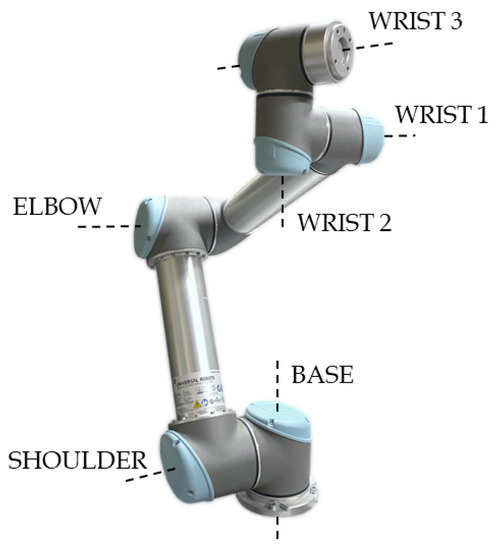
\includegraphics[width=0.4\textwidth]{2-arm.jpg}
    \captionsetup{justification=centering}
    \caption{\textit{Labeled structure of the UR3 robotic arm, showing the six rotational joints: Base, Shoulder, Elbow, Wrist 1, Wrist 2, and Wrist 3. \cite{robotics12030071}}}
    \label{fig:2-arm}
\end{figure}

\begin{center}
    Figure \ref{fig:2-arm} illustrates the UR3 robotic arm, which comprises six revolute joints: Base, Shoulder, Elbow, Wrist 1, Wrist 2, and Wrist 3. The corresponding joint configurations and their operating ranges, each allowing a rotation of $\pm 360^\circ$, are detailed in Table \ref{tab:arm}.
\end{center}

\renewcommand{\arraystretch}{1.1}
\begin{table}[h]
    \centering
    \caption{\textit{UR3 Robotic Arm Joint Movements and Corresponding Operating Ranges.}}
    \begin{tabular}{|C{7cm}|C{4cm}|}
        \hline
        \rowcolor[HTML]{d9d9d9}  % Dark grey color
        \textcolor{black}{\textbf{Robotic Arm Axis Movement}} & \textcolor{black}{\textbf{Operating Range}} \\
        \hline
        Base   & $\pm 360^\circ$   \\
        \hline
        Shoulder     & $\pm 360^\circ$     \\
        \hline
        Elbow & $\pm 360^\circ$ \\
        \hline
        Wrist 1   & $\pm 360^\circ$   \\
        \hline
        Wrist 2   & $\pm 360^\circ$ \\
        \hline
        Wrist 3      & $\pm 360^\circ$   \\
        \hline
    \end{tabular}
    \label{tab:arm}
\end{table}


\newpage
\section{Integration}
\subsection{Software Architecture and Communications Framework}
The software integration for the system implements a communication framework connecting three primary components: the vision system, the UR3 robotic arm, and the conveyor belt control system. This integration enables real-time detection of boxes moving along the conveyor and robotic arm movements to retrieve the targets.
\subsection{TCP Communication Architecture}
The system utilizes Transmission Control Protocol (TCP) socket connections to establish reliable communication channels between different components. This architecture ensures correctness within the transmitted data between different systems:
\begin{itemize}
    \item A TCP connection to the vision system (IP: 10.10.1.10, Port: 2024) receives continuous coordinate data of detected boxes
    \item A TCP connection to the UR3 robot controller (IP: 10.10.0.14, Port: 30003) sends movement commands in real-time
    \item A TCP connection to the gripper controller (IP: 10.10.0.14, Port: 63352) controls opening and closing actions
    \item A TCP connection to a local conveyor controller (IP: 10.10.0.98, Port: 2002) manages conveyer belt operations
\end{itemize}

The choice of TCP over alternatives like UDP ensures reliable and correct data delivery with error checking, which is critical for the precision required in robotic picking applications.

\subsection{Vision System Integration}

\begin{enumerate}
    \item \textbf{Data Reception and Parsing:} The system receives coordinate strings from the vision system in a custom format with sides delimited by "/" characters and coordinates by commas. This data provides the position of the box's left, right, top, and bottom edges.
    \item \textbf{Motion Analysis:} The software implements a simple but effective motion tracking algorithm that:
    \begin{itemize}
        \item First, record the initial y-position when a box is first detected. Next, calculate the change in position between successive frames and save these values in a list (see Fig. \ref{fig:7-diff}).       
        \item After a predetermined number of frames, compute the average change across all frames. Then convert the pixel displacements to physical distances using a calibration constant of 0.2 m per frame, and calculate the resulting speed in meters per second (see Fig. \ref{fig:8-yspeed}).
        \item Finally, use the obtained speed to determine the grab-offset position via \begin{math} s=v*t \end{math}, as shown in Fig. \ref{fig:9-calc}.
    \end{itemize}

\begin{figure} [!ht]
    \centering
    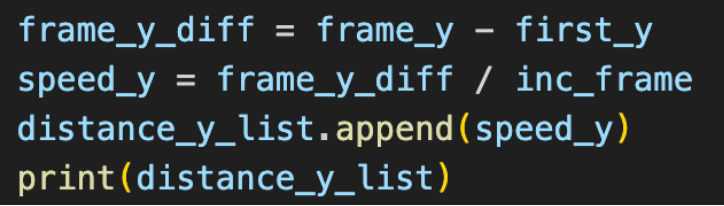
\includegraphics[width=0.5\textwidth]{7-diff.png}
    \captionsetup{justification=centering}
    \caption{\textit{Code to calculate y difference in each frame}}
    \label{fig:7-diff}
\end{figure}

\begin{figure} [!ht]
    \centering
    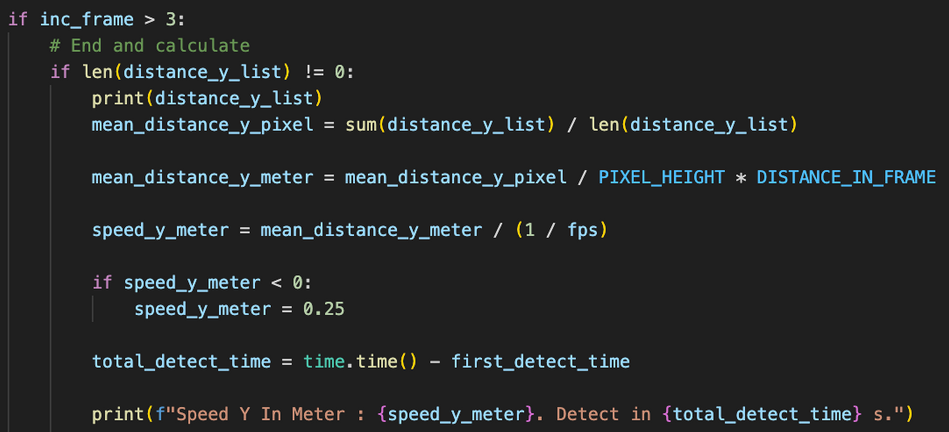
\includegraphics[width=0.9\textwidth]{8-yspeed.png}
    \captionsetup{justification=centering}
    \caption{\textit{Code to calculate y speed}}
    \label{fig:8-yspeed}
\end{figure}

\begin{figure} [!ht]
    \centering
    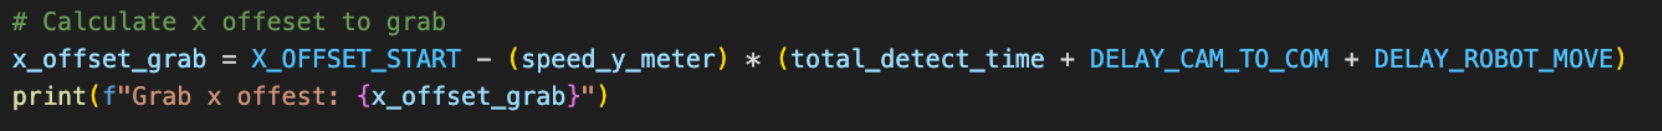
\includegraphics[width=0.9\textwidth]{9-calc.png}
    \captionsetup{justification=centering}
    \caption{\textit{Code to calculate offset to grab}}
    \label{fig:9-calc}
\end{figure}
\newpage
    \item \textbf{Position Estimation:} The system calculates where to position the gripper by:
    \begin{itemize}
        \item Determining the center point between the left and right edges of the box
        \item Converting pixel coordinates to physical distances using a calibration constant
        \item Applying offsets to account for the camera's perspective
    \end{itemize}
\end{enumerate}

This approach provides sufficient information to predict where the box will be when the robot reaches it, compensating for the inherent delays in the system.

\subsection{UR3 Robot Arm Control}
The control of the UR3 robotic arm is implemented through a custom Robot class that abstracts the complexities of robot programming:

\begin{enumerate}
    
    \item \textbf{Position Control:} The robot is controlled through absolute pose commands (movel) that specify the end-effector's position and orientation in Cartesian space. This approach simplifies the trajectory planning by delegating inverse kinematics calculations to the UR3 controller.
    
    \item \textbf{Home Position:} A predefined home position is established as a reference point for all movements, with additional movements defined relative to this position using the $move\_wrt\_home$ method.

    \item \textbf{Timing Management:} The system accounts for various delays in the control loop:
    
    \begin{itemize}
        \item Camera-to-computer delay (0.25 seconds)
        \item Robot movement delay (0.35 seconds)
        \item These delays are factored into the position calculations to compensate for the conveyor belt's continuous motion 
    \end{itemize}

    \item \textbf{Calibration Parameters:} The code incorporates calibration constants to translate between pixel coordinates and physical distances, ensuring accurate positioning of the robot arm.

\end{enumerate}

\subsection{Synchronized Operation Logic}
The integration synchronizes all components through a main control loop that follows a sequential process:
\begin{enumerate}
    \item \textbf{Initialization:} The system initializes all connections and sets the robot to its home position.
    \item \textbf{Conveyor Activation:} The conveyor belt is activated at a specified speed (20 units).
    \item \textbf{Control Loop:} The control loop continuously:
    \begin{itemize}
        \item Receives vision data
        \item Processes box positions to detect new boxes and track movement
        \item Calculates box velocity and predicts future positions
        \item Prepares the gripper based on detected box size
        \item Executes picking maneuvers at calculated intercept points
        \item Returns to home position after successful picks
    \end{itemize}
\end{enumerate}

The loop implements timing constraints to ensure that operations occur within the narrow window available for successful picking. The system employs a predictive approach where the robot is commanded to move to where the box will be, rather than where it currently is, accounting for system delays.

\subsection{Performance Considerations}
Several performance optimizations are evident in the implementation:
\begin{itemize}
    \item \textbf{Frame Rate Monitoring:} The system calculates frames per second (fps) to maintain awareness of the vision system's processing speed, which affects motion calculations.
    \item \textbf{Adaptive Positioning:} The grabbing position is dynamically adjusted based on the calculated speed of the conveyor belt and the system's processing delays.
    \item \textbf{Error Bounds:} The code includes constraints to keep motion parameters within safe limits, preventing extreme movements that could damage the system.
\end{itemize}

The integration balances complexity with reliability, creating a system capable of precisely timing robotic movements to intercept moving objects on a conveyor belt—a challenging task that requires precise coordination between vision, robot control, and motion prediction.

\newpage
\section{Results \& Conclusion}
This project successfully demonstrated the effective integration of robotics and computer vision to demonstrate the efficient \& quick pick of a box. Utilizing the UR3 robotic arm and NI Vision Builder, the system reliably detected, tracked, and manipulated moving boxes on a conveyor belt through precise synchronization of hardware and software components. The employment of TCP/IP communication protocols facilitated accurate real-time data exchange. The custom-developed Python control logic, incorporating predictive positioning and adaptive adjustments, effectively compensated for system delays. As a result, our team achieved the fastest pick-up time among all groups, 2.7 seconds from the moment the box was placed on the conveyor to returning to the home position, highlighting the efficiency of our system.

\newpage
\addcontentsline{toc}{section}{References}
\bibliographystyle{IEEEtran}
\bibliography{references}

\end{document}
